\documentclass[25pt, a0paper, portrait, margin=0mm, innermargin=20mm,
blockverticalspace=2mm, colspace=20mm, subcolspace=0mm]{tikzposter} %Default values for poster format options.

\usepackage[utf8]{inputenc}
\usepackage[scaled]{helvet}
\renewcommand\familydefault{\sfdefault}
\usepackage[T1]{fontenc}
\usepackage{wrapfig}
\usepackage{setspace}
\usepackage{multicol}
\setlength{\columnsep}{1.5cm}
\usepackage{xspace}
\usepackage{tikz}
\usepackage{lipsum}

\tikzposterlatexaffectionproofoff
\usetheme{Default}

\definecolor{text}{HTML}{e0e4f7}
\definecolor{background}{HTML}{111116}
\definecolor{boxes}{HTML}{2a2a32}
\definecolor{unired}{HTML}{a51e37}

\colorlet{blocktitlefgcolor}{text}
\colorlet{backgroundcolor}{background}
\colorlet{blocktitlebgcolor}{background}
\colorlet{blockbodyfgcolor}{text}
\colorlet{innerblocktitlebgcolor}{background}
\colorlet{innerblocktitlefgcolor}{text}
\colorlet{notefrcolor}{text}
\colorlet{notefgcolor}{background}
\colorlet{notebgcolor}{background}


% Title setup
\settitle{
% Rearrange the order of the minipages to e.g. center the title between the logos
\begin{minipage}[c]{0.8\paperwidth}
%    \centering
    \vspace{2.5cm}\hspace{1.5cm}
    \color{text}{\Huge{\textbf{\@title}} \par}
    \vspace*{2em}\hspace{1.5cm}
    \color{text}{\LARGE \@author \par}
    \vspace*{2em}\hspace{1.5cm}
    \color{text}{\Large \@institute}
    \vspace{2.5cm}
\end{minipage}
\begin{minipage}[c]{0.2\paperwidth}
    \centering
    % \vspace{1cm}
    \hspace{-10cm}
    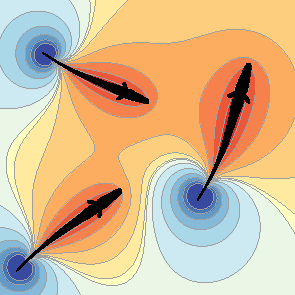
\includegraphics[width=0.8\linewidth]{figs/efishlogo.pdf}
\end{minipage}}
% \begin{minipage}[c]{0.2\paperwidth}
%     \vspace{1cm}\hspace{1cm}
%     \centering
%     \includegraphics[width=\linewidth]{example-image-a}
% \end{minipage}}

% define title style with background box (currently white)
\definetitlestyle{sampletitle}{
    width=841mm,
    roundedcorners=0,
    linewidth=0pt,
    innersep=15pt,
    titletotopverticalspace=0mm,
    titletoblockverticalspace=5pt
}{
    \begin{scope}[line width=\titlelinewidth,
        rounded corners=\titleroundedcorners]
    \draw[fill=text, color=boxes]
    (\titleposleft,\titleposbottom)
    rectangle
    (\titleposright,\titlepostop);
    \end{scope}
}

% define coustom block style for visible blocks
\defineblockstyle{GrayBlock}{
    titlewidthscale=1,
    bodywidthscale=1,
    % titlecenter,
    titleleft,
    titleoffsetx=0pt,
    titleoffsety=-30pt,
    bodyoffsetx=0pt,
    bodyoffsety=-40pt,
    bodyverticalshift=0mm,
    roundedcorners=25,
    linewidth=1pt,
    titleinnersep=20pt,
    bodyinnersep=38pt
}{
    \draw[rounded corners=\blockroundedcorners, inner sep=\blockbodyinnersep,
          line width=\blocklinewidth, color=background,
          top color=boxes, bottom color=boxes,
          ]
      (blockbody.south west) rectangle (blockbody.north east); %
    \ifBlockHasTitle%
        \draw[rounded corners=\blockroundedcorners, inner sep=\blocktitleinnersep,
          top color=background, bottom color=background,
          line width=2, color=background, %fill=blocktitlebgcolor
          ]
      (blocktitle.south west) rectangle (blocktitle.north east); %
    \fi%
}
\newcommand\myblock[3][GrayBlock]{\useblockstyle{#1}\block{#2}{#3}\useblockstyle{Default}}

% Define blockstyle for tranparent block
\defineblockstyle{TranspBlock}{
    titlewidthscale=0.99,
    bodywidthscale=0.99,
    titleleft,
    titleoffsetx=15pt,
    titleoffsety=-40pt,
    bodyoffsetx=0pt,
    bodyoffsety=-40pt,
    bodyverticalshift=0mm,
    roundedcorners=25,
    linewidth=1pt,
    titleinnersep=20pt,
    bodyinnersep=38pt
}{
    \draw[rounded corners=\blockroundedcorners, inner sep=\blockbodyinnersep,
          line width=\blocklinewidth, color=background,
          top color=background, bottom color=background,
          ]
      (blockbody.south west) rectangle (blockbody.north east); %
    \ifBlockHasTitle%
        \draw[rounded corners=\blockroundedcorners, inner sep=\blocktitleinnersep,
          top color=background, bottom color=background,
          line width=2, color=background, %fill=blocktitlebgcolor
          ]
      (blocktitle.south west) rectangle (blocktitle.north east); %
    \fi%
}
\renewcommand\myblock[3][TranspBlock]{\useblockstyle{#1}\block{#2}{#3}\useblockstyle{Default}}


\begin{document}

\renewcommand{\baselinestretch}{1}
\title{\parbox{1600pt}{Detecting chirps based on dynamic filtering for the \\ analysis of social interactions in weakly electric fish}}
\author{Sina Prause, Alexander Wendt, and Patrick Weygoldt}
\institute{Supervised by Till Raab \& Jan Benda, Neuroethology Lab, University of Tuebingen}
\usetitlestyle[]{sampletitle}
\maketitle
\renewcommand{\baselinestretch}{1.4}

\begin{columns}
\column{0.4}
\myblock[TranspBlock]{Introduction}{
    \textbf{Chirps} are the most common communication signals in weakly electric fish. They are characterized by \textbf{short frequency excursions} and are emitted during various social contexts. It is nearly impossible to reliably \textbf{detect and assign} chirps in freely interacting fish using only a Fourier transform. To overcome these limits, we developed a new method of \textbf{dynamic feature extraction} and classification.
    \vspace{0cm}
    \begin{tikzfigure}[]
        \label{griddrawing}
        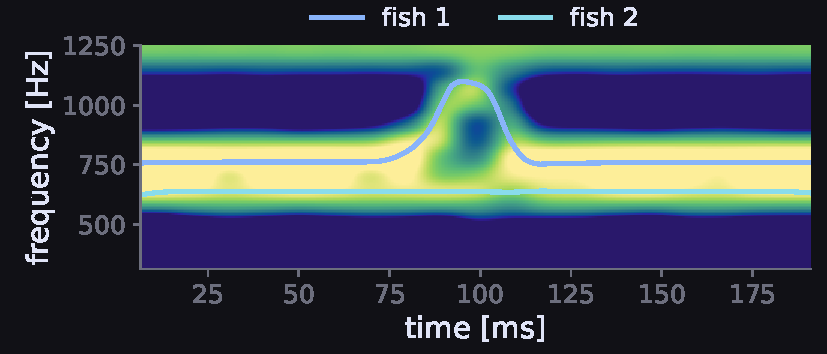
\includegraphics[width=\linewidth]{figs/introplot}
    \end{tikzfigure}
}
\myblock[TranspBlock]{Chirp Detection Algorithm}{
    \begin{tikzfigure}[]
        \label{fig:alg1}
        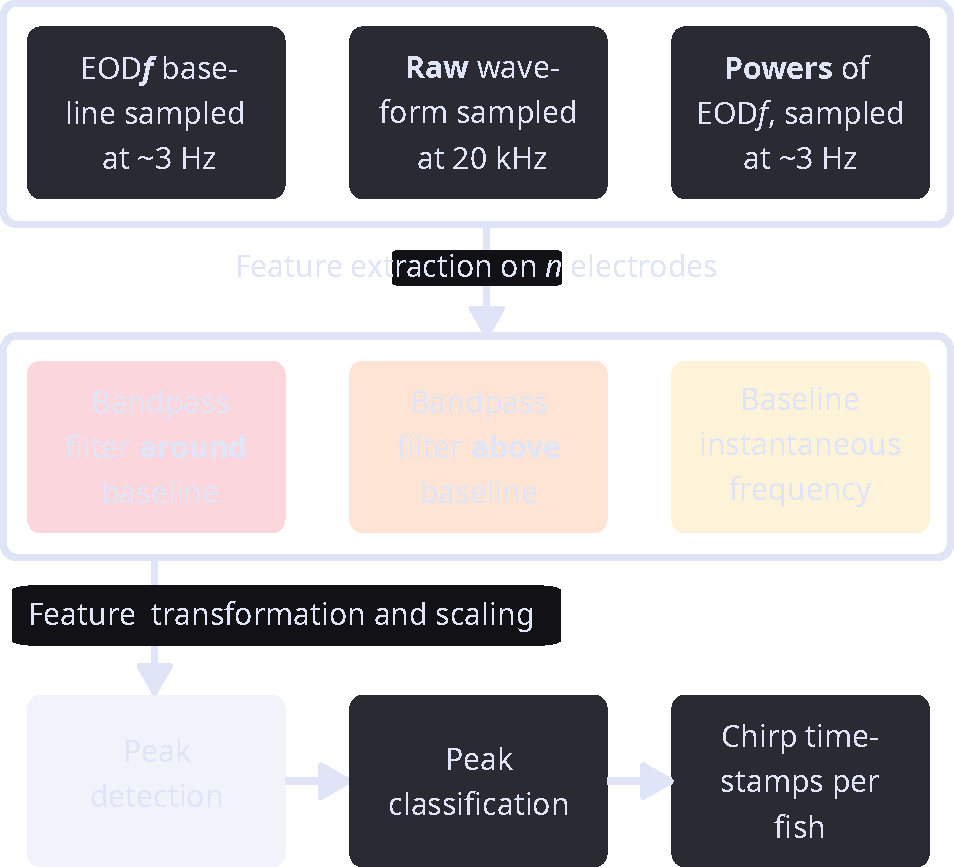
\includegraphics[width=0.9\linewidth]{figs/algorithm1}
    \end{tikzfigure}
    \vspace{0cm}
    \begin{tikzfigure}[]
        \label{fig:alg2}
        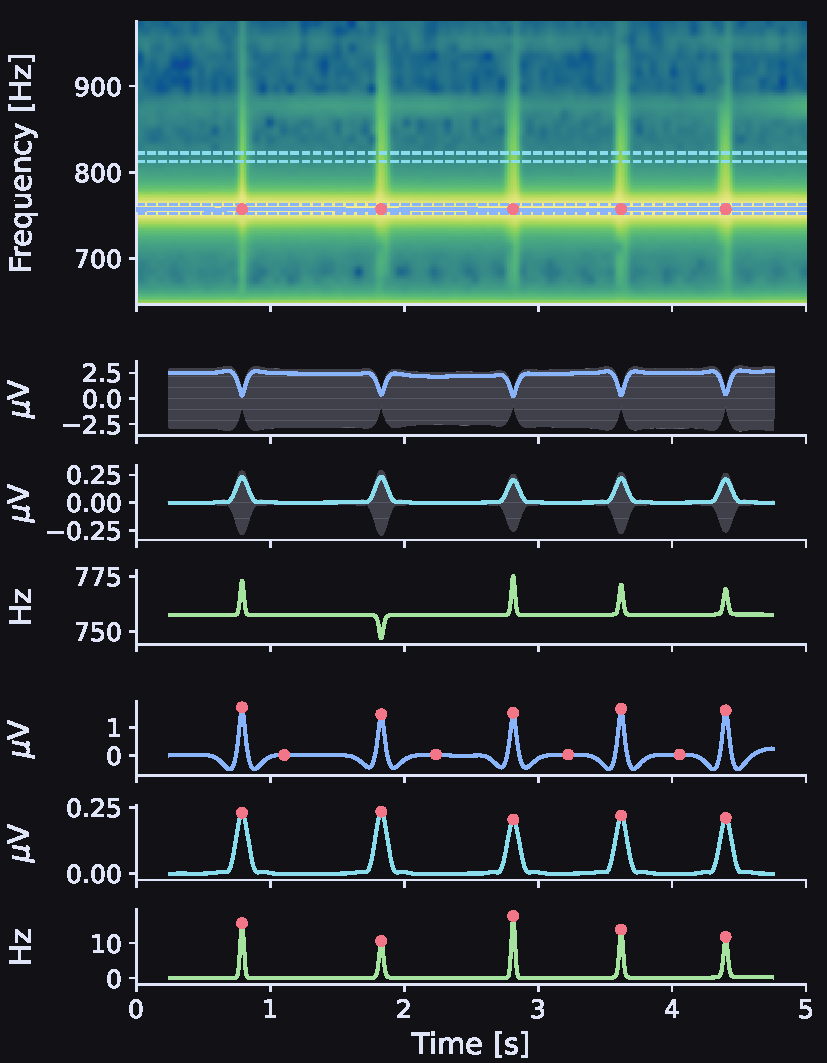
\includegraphics[width=1\linewidth]{figs/algorithm}
    \end{tikzfigure}
    \vspace{0cm}
}

\column{0.6}
\myblock[TranspBlock]{Chirps in dyadic competitions (Data by Till Raab, 2020)}{
    \vspace{-2.75cm}
    \begin{tikzfigure}[]
        \label{fig:example_b}
        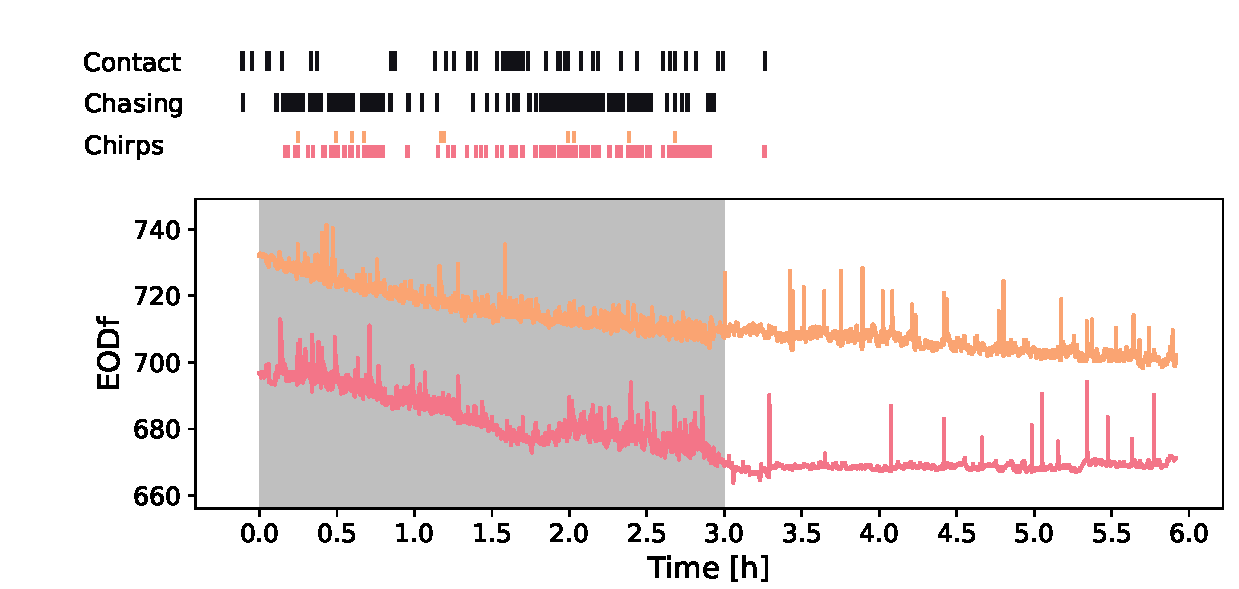
\includegraphics[width=\linewidth]{figs/timeline.pdf}
    \end{tikzfigure}
    \noindent
    \begin{multicols}{2}
        \begin{itemize}
            % \setlength\itemsep{0.5em}
            \item The electric behavior of two fish competing for one shelter were recorded in a light and dark condition.
            \item Using video recordings, behavior was classified as chasings or physical contacts.
        \end{itemize}
    \end{multicols}

    \vspace{-2cm}
    \noindent
    \begin{tikzfigure}[]
        \label{fig:example_b}
        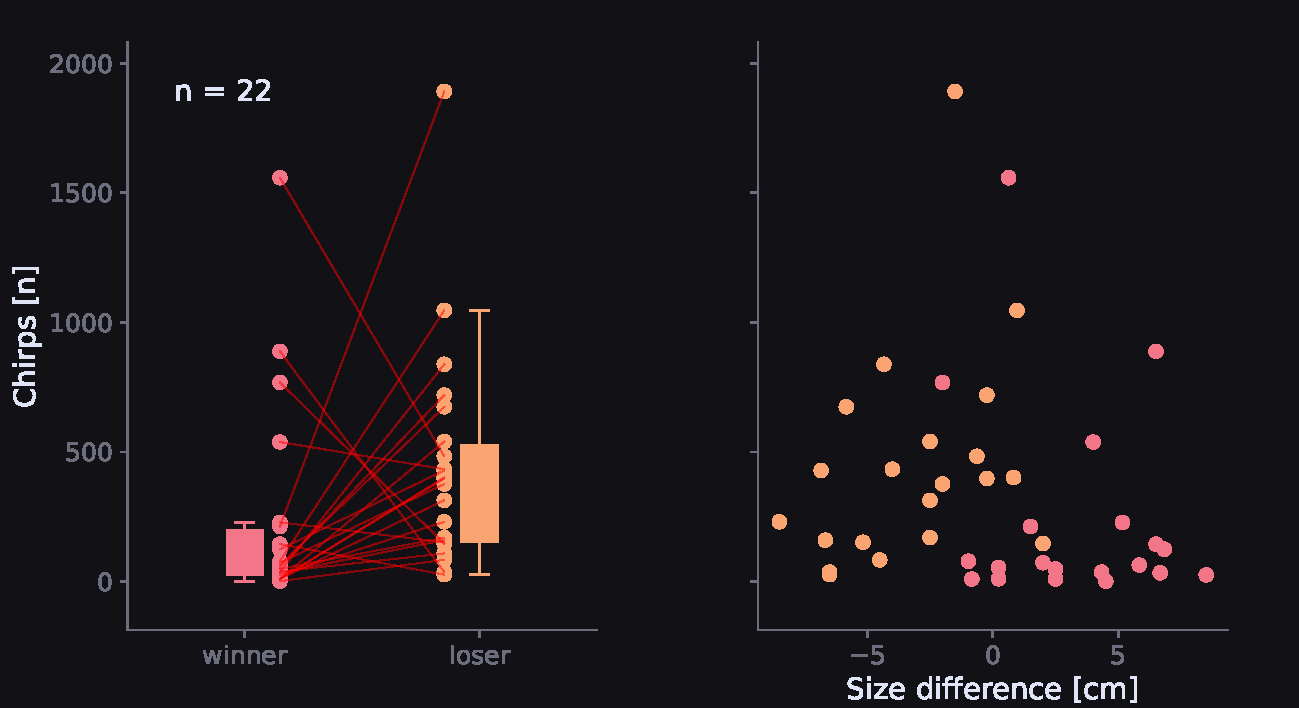
\includegraphics[width=\linewidth]{figs/chirps_winner_loser.pdf}
    \end{tikzfigure}
    \noindent
    \begin{multicols}{2}
        \begin{itemize}
            \item Losers tend to chirp more.
            \item Larger fish usually win. The smaller the size difference the more chirps are emitted.
            \columnbreak
            \item EOD frequency has no effect on the competition outcome and the chirp rate.
        \end{itemize}
    \end{multicols}
}

\myblock[TranspBlock]{Chirps emitted by loser fish might stop chasing events}{
    \vspace{-1.2cm}
    \begin{minipage}{0.6666\linewidth}
        \begin{tikzfigure}[]
            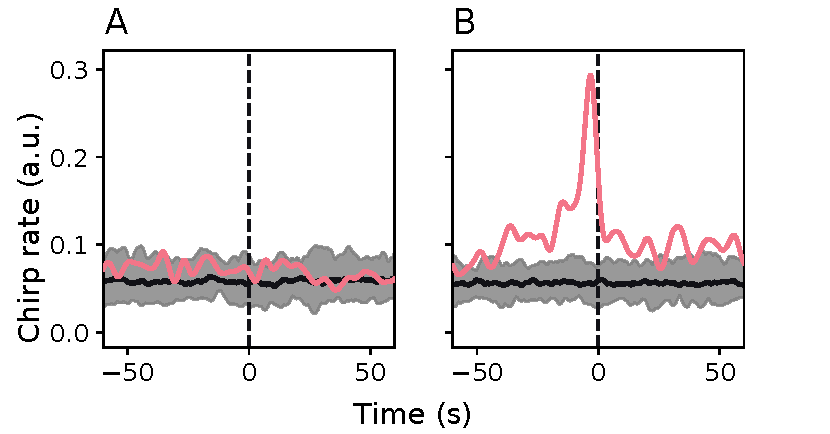
\includegraphics[width=1.1\linewidth]{figs/kde.pdf}
        \end{tikzfigure}
    \end{minipage}
        \begin{minipage}{0.3333\linewidth}
            \begin{tikzfigure}[]
                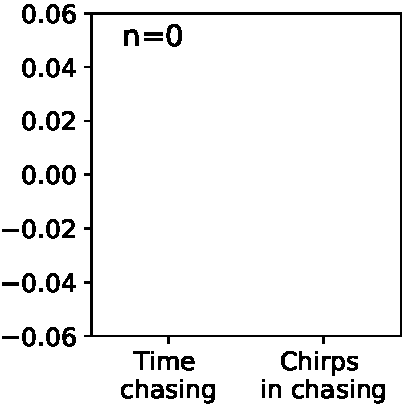
\includegraphics[width=1\linewidth]{figs/chirps_in_chasing.pdf}
            \end{tikzfigure}
    \end{minipage}
    \noindent
    \begin{multicols}{2}
        \begin{itemize}
            \item In most cases there is no correlation between chirping and chasing- or physical contact events.
            \item The chirp rate during chasings only increases for some dyads.
        \end{itemize}
    \end{multicols}
}

\myblock[GrayBlock]{Conclusion}{
    \begin{itemize}
        \setlength\itemsep{0.5em}
        \item First tests indicate that our algorithm is able to detect chirps in recordings of multiple fish.
        \item In some cases the chirp rate drastically increases before chasing stops.
        \item Behavioral analysis needs to consider more variables, such as sex, size, and interindividual differences in chirping behavior.
    \end{itemize}
    \vspace{0.2cm}
    }
    \end{columns}

\node [above right,
    text=white,
    outer sep=45pt,
    minimum width=\paperwidth,
    align=center,
    draw,
    fill=boxes,
    color=boxes] at (-43.6,-61) {
        \textcolor{white}{
    \normalsize Contact: \{name\}.\{surname\}@student.uni-tuebingen.de}};

\end{document}
